\chapterimage{band1.png}
\chapter{Iteração}\label{cap:iteraccao}

A maior parte dos programas repetem várias vezes as mesmas operações sobre os mesmos dados ou sobre dados
diferentes. 
Muitas acções que realizamos na vida real são, de facto, a repetição de uma acção mais básica. Por exemplo, subir escadas: a acção mais básica é subir um degrau; esta operação é repetida até chegarmos ao final das escadas. Poderiamos pensar que a acção básica não é a mesma repetida, afinal, não subimos sempre o mesmo degrau! Mas nestes casos, o que interessa é que o conjunto de acções que a pessoa efectua para subir um degrau: levantar a perna, apoiar o pé, elevar o corpo e apoiar o outro pé, são sempre os mesmos independentemente do degrau estar mais acima ou mais abaixo.

Também em programação acontece frequentemente necessitarmos de repetir várias vezes a mesma acção, um determinado número de vezes, ou enquanto determinada condição for verdadeira.

Para repetirmos um conjunto de operações utilizamos as chamadas instruções de \emph{iteração}, ou \emph{ciclos}.

Existem duas classes de ciclos: ciclos que executam um número pré-determinado de vezes e ciclos que executam enquanto determinada condição não for satisfeita. Estas classes de ciclos têm analogias com situações da vida real. Na situação de ``subir a escada'', normalmente não sabemos à partida quantos degraus vamos ter de subir, mas sabemos que temos de continuar a subir degraus enquanto eles não acabarem, ou enquanto não chegarmos ao nosso piso -- este seria um ciclo que executa enquanto determinada condição não for satisfeita. Numa outra situação, por exemplo no caso em que vamos comprar laranjas ao supermercado, normalmente sabemos quantas laranjas vamos querer comprar. Neste caso colocamos laranjas no saco até chegarmos ao número pretendido -- este ciclo executa um número pré-determinado de vezes.

Para a primeira classe de ciclos existem duas variantes em programação: o ciclo \texttt{while} -- executa zero ou mais vezes, enquanto uma condição for verdadeira; e o ciclo \texttt{do} -- executa uma ou mais vezes, enquanto uma condição for verdadeira; 

Para a segunda classe de ciclos existe o ciclo \texttt{for} -- utilizado principalmente para iterar um número pré-determinado de vezes; 


\section{\texttt{while}}
A Figura~\ref{fig:enquanto} mostra o diagrama de fluxo do ciclo \texttt{while}.
\begin{figure}[!h]
	\centering
		\includegraphics[width=5cm]{images/enquanto.eps}
	\caption{\texttt{while} -- diagrama de fluxo}
	\label{fig:enquanto}
\end{figure}

A sintaxe deste ciclo é a seguinte:
\begin{lstlisting}
while (<condição>) {
    <acções>
}
\end{lstlisting}

Quando o programa chega à primeira linha do ciclo, a condição é testada. Se a condição for verdadeira, então o programa segue para a primeira linha das acções. Quando chegar à última linha das acções, o programa volta automaticamente à primeira linha do ciclo e testa novamente a condição. Se a condição for falsa, então o programa segue para a instrução a seguir ao final do ciclo. Uma vez que a condição é testada no início do  ciclo, pode acontecer que o ciclo não execute nenhuma vez: se a condição for falsa logo da primeira vez.

O exemplo seguinte exemplifica o uso deste ciclo para escrever os números de 0 a 10:
\begin{lstlisting}
int i = 0;
while (i <= 10) {
    print(i);
    i = i + 1;
}
\end{lstlisting}
Neste exemplo, a condição para execução do ciclo é a variável \texttt{i} ser menor ou igual a 10. Se isto for verdade, então o programa escreve o valor de \texttt{i} -- com a instrução \texttt{print()} -- e aumenta o valor da variável. No exemplo, a variável \texttt{i} foi inicializada a zero. Se a inicializassemos com um valor superior a 10, o ciclo não executava nenhuma iteração%
\footnote{Uma \emph{iteracção} é uma execução das acções de um ciclo.}%
:
\begin{lstlisting}
int i = 15;
while (i <= 10) {
    print(i);
    i = i + 1;
}
\end{lstlisting}
Neste caso, a condição é falsa logo à partida.


\section{\texttt{do}}
O ciclo \texttt{do} é uma variante do ciclo anterior.
A Figura~\ref{fig:fazer} mostra o diagrama de fluxo do ciclo \texttt{do}.
\begin{figure}[!h]
	\centering
		\includegraphics[width=5cm]{images/fazer.eps}
	\caption{\texttt{do} -- diagrama de fluxo}
	\label{fig:fazer}
\end{figure}

A diferença para o ciclo anterior (\texttt{while}) é que, no ciclo \texttt{do}, a condição é testada apenas no final do ciclo. Isto significa que as acções deste ciclo executam sempre, pelo menos uma vez. A sintaxe geral deste ciclo é a seguinte:
\begin{lstlisting}
do {
    <acções>
} while (<condição>);
\end{lstlisting}

Como exemplo de utilização vamos reescrever o exemplo anterior (escrita dos números de 0 a 10) com o ciclo \texttt{do}:
\begin{lstlisting}
int i = 0;
do {
    print(i);
    i = i + 1;
} while (i <= 10);
\end{lstlisting}
Este ciclo executa exactamente o mesmo que o exemplo anterior. No entanto, se agora inicializarmos a variável \texttt{i} a 15, como fizemos anteriormente:
\begin{lstlisting}
int i = 15;
do {
    print(i);
    i = i + 1;
} while (i <=10);
\end{lstlisting}
Verificamos que o programa escreve o valor ``15''. Isto acontece porque o ciclo \texttt{do} executa sempre pelo menos uma vez. Apenas depois da primeira iteracção do ciclo é que a condição é testada.

\section{\texttt{for}}
Este ciclo corresponde à classe de ciclos utilizada para iterar um número pré-determinado de vezes.
O diagrama de fluxo do ciclo \texttt{for} está exemplificado na Figura~\ref{fig:para}.
\begin{figure}[h]
	\centering
		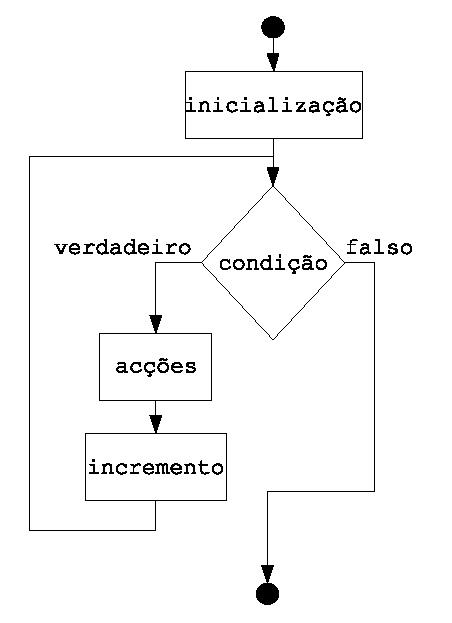
\includegraphics[width=5cm]{images/para.eps}
	\caption{\texttt{for} -- diagrama de fluxo}
	\label{fig:para}
\end{figure}
A sintaxe deste ciclo é um bocado mais complexa do que as anteriores:
\begin{lstlisting}
for (<inicialização>;<condição>;<incremento>) {
    <acções>
}
\end{lstlisting}

O ciclo \texttt{for} utiliza uma variável para contar o número de vezes que já executou. Essa variável pode ser uma qualquer variável numérica do nosso programa que deverá ser inicializada na secção <inicialização> do ciclo. Normalmente utilizamos nomes especiais para estas variáveis: \texttt{i}%
\footnote{O nome \texttt{i} para estas variáveis deve-se ao facto de na maioria das vezes, estas variáveis servirem de \textbf{í}ndices para vectores.}%
, \texttt{j}, \texttt{k}, etc.

Em <condição>, colocamos a condição de paragem do ciclo. Normalmente, esta condição toma a forma de \texttt{i < x;}, em que x é o número de vezes que queremos executar o ciclo.

A secção <incremento> serve para aumentar o valor da variável de forma a avançarmos. Na maior parte das vezes utilizamos: \texttt{i = i + 1;}%
\footnote{Irão ver muitas vezes expressões como \texttt{i++;} em vez de \texttt{i = i + 1;}. As duas são equivalentes.}. 
 para incrementar uma unidade.


Assim para escrevermos os números de 0 a 10, fariamos:
\begin{lstlisting}
int i;
for (i = 0; i <= 10; i = i + 1) {
    print (i);
}
\end{lstlisting}
Reparem que, neste caso, não temos de incrementar a variável no corpo do ciclo. Isto é feito na secção de incremento.



\section{Tipos de variáveis complexos}
Até agora temos vindo a utilizar apenas tipos de variáveis simples. Estas variáveis podem guardar um valor de cada vez -- são ``gavetas'' que apenas podem ter um valor. 

Os vectores são como gavetas sequenciais que podem ser referidas através de um nome e um índice. O nome identifica o conjunto de gavetas, enquanto que o índice identifica a gaveta dentro do conjunto. Deste modo podemos ter vários conjuntos de gavetas com nomes diferentes.
O nome do conjunto de gavetas não é mais do que o nome da variável que definirmos no nosso programa.

Os vectores permitem-nos agrupar dados do mesmo tipo de uma forma mais prática do que se definissemos uma variável para cada valor. Por exemplo, vamos supor que necessitamos de guardar as idades de todos os alunos de uma turma. Os alunos e respectivas idades são:
\begin{center}
\begin{tabular}{ll}
Nome & Idade\\
\hline
Pedro 	& 20 \\
Rui			& 19 \\
Osvaldo & 19 \\
Guilherme	& 20\\
Romão			& 18\\
Ana				& 19\\
Maria			& 18\\
Anacleto	& 20\\
Carlos		& 21\\
António		& 17\\
Osório		& 18\\
Manuela		& 17\\
Ulmira	 	& 18\\
Luís			& 20\\
Tibério		& 19\\
Irina			& 20\\
Mafalda		& 18\\
Emília		& 19\\
Diogo			& 20\\
Isabel		& 19\\
Aleixo		& 20\\
\end{tabular}
\end{center}
Uma possível solução para este problema seria utilizar tantas variáveis como número de alunos:
\begin{lstlisting}
int pedro     = 20;
int rui       = 19;
int osvaldo   = 19;
int guilherme = 20;
int romão     = 18;
int ana       = 19;
int maria     = 18;
int anacleto  = 20;
int carlos    = 21;
int antónio   = 17;
int osório    = 18;
int manuela   = 17;
int ulmira    = 18;
int luís      = 20;
int tibério   = 19;
int irina     = 20;
int mafalda   = 18;
int emília    = 19;
int diogo     = 20;
int isabel    = 19;
int aleixo    = 20;
\end{lstlisting}
E agora, se quisessemos calcular a médias das idades?:
\begin{lstlisting}
float media;

media = (pedro + rui + osvaldo + guilherme + romão + ana + maria + 
        anacleto + carlos + antónio + osório + manuela + ulmira + 
        luís + tibério + irina + mafalda + emília + diogo + isabel + 
        aleixo)/21;
\end{lstlisting}
Como devem ter percebido é muito trabalhoso utilizar tantas variáveis... 

Se reparem bem, todas as variáveis guardam o mesmo tipo de dados: uma idade.
Uma forma mais prática de resolver o problema seria utilizar um vector:
\begin{lstlisting}
int idades[];

idades = new int[21]; 

idades[0]  = 20; // pedro
idades[1]  = 19; // rui  
idades[2]  = 19; // osvaldo
idades[3]  = 20; // guilherme 
idades[4]  = 18; // romão     
idades[5]  = 19; // ana     
idades[6]  = 18; // maria   
idades[7]  = 20; // anacleto  
idades[8]  = 21; // carlos   
idades[9]  = 17; // antónio 
idades[10] = 18; // osório    
idades[11] = 17; // manuela  
idades[12] = 18; // ulmira    
idades[13] = 20; // luís     
idades[14] = 19; // tibério 
idades[15] = 20; // irina 
idades[16] = 18; // mafalda 
idades[17] = 19; // emília 
idades[18] = 20; // diogo 
idades[19] = 19; // isabel 
idades[20] = 20; // aleixo 

int i;
float media = 0;

for (i = 0; i < 21; i = i + 1) {
    media = media + idades[i];
}
media = media/21;
\end{lstlisting}
O programa anterior cria um vector com 21 posições (do tipo \texttt{int}) e inicializa-as com as idades dos alunos.
O ciclo final serve para somar todas as idades (para no fim, calcular a média).

Esta forma de utilizar variáveis é muito mais prática do que a versão anterior, porque é muito mais flexível. Neste caso particular para a inicialização, continua a ser necessário um conjunto de várias linhas de código. Mas todas as outras operações ficam facilitadas pela possibilidade de utilização de um ciclo para percorrer cada posição do vector. Para mostrar mais um exemplo da flexibilidade dos vectores, vamos supor que precisavamos de somar 5 anos a cada idade. Na primeira versão teriamos algo como:
\begin{lstlisting}
pedro     = pedro     + 5;
rui       = rui       + 5;
osvaldo   = osvaldo   + 5;
guilherme = guilherme + 5;
romão     = romão     + 5;
ana       = ana       + 5;
maria     = maria     + 5;
anacleto  = anacleto  + 5;
carlos    = carlos    + 5;
antónio   = antónio   + 5;
osório    = osório    + 5;
manuela   = manuela   + 5;
ulmira    = ulmira    + 5;
luís      = luís      + 5;
tibério   = tibério   + 5;
irina     = irina     + 5;
mafalda   = mafalda   + 5;
emília    = emília    + 5;
diogo     = diogo     + 5;
isabel    = isabel    + 5;
aleixo    = aleixo    + 5;
\end{lstlisting} 

Na versão com vectores bastava:
\begin{lstlisting}
int i;
for (i = 0; i < 21; i = i + 1) {
    idades[i] = idades[i] + 5;
}
\end{lstlisting}

Algumas das linhas de código usadas nos exemplos anteriores precisam de explicação. É isso que vamos ver nas secções seguintes.

\subsection{Declarar e Inicializar Vectores}
A linha
\begin{lstlisting}
int idades[];
\end{lstlisting}
declara um vector de inteiros. Esta linha apenas indica ao programa que vamos utilizar uma variável com o nome \texttt{idades} e que essa variável é um vector. Para o programa poder reservar memória para esta variável falta um pedaço de informação importante: o tamanho do vector, ou seja, quantas posições o vector irá conter.

Para indicarmos ao programa que vamos precisar de x posições temos de utilizar uma \emph{keyword} especial -- \texttt{new}:
\begin{lstlisting}
idades = new int[21]; 
\end{lstlisting}
Com esta linha indicamos ao programa que o nosso vector (\texttt{idades}) precisa de guardar 21 números inteiros.

A sintaxe geral para reservar memória para um vector é a seguinte:
\begin{lstlisting}
nomeVariavel = new tipoVariavel[tamanhoVector];
\end{lstlisting}

Para declarar e reservar espaço para um vector de 100 booleanos, fariamos:
\begin{lstlisting}
boolean passouTeste[];

passouTeste = new boolean[100];
\end{lstlisting}

\subsection{Percorrer Vectores}
Uma das grandes vantagens dos vectores é o facto de podermos realizar a mesma operação sobre cada um dos elementos desse vector. A melhor forma de fazermos isto é através de um ciclo:
\begin{lstlisting}
int posicaoY[] = new int[100];
int i;

for (i = 0; i < 100; i = i + 1) {
    posicaoY[i] = posicaoY[i] + 1;
}
\end{lstlisting}

Basicamente, o que temos de fazer para aceder a uma posição do vector é utilizar a sintaxe \texttt{nomeVector[indice]}.
Por exemplo para aceder à primeira posição%
\footnote{A primeira posição de um vector, em Processing, é a posição 0 (zero). Nalgumas linguagens de programação a primeira posição dos vectores é a posição 1 (um).}%
:
\begin{lstlisting}
int pedro;

pedro = idades[0];
\end{lstlisting}

O valor utilizado como índice do vector pode ser uma variável, ou uma expressão, cujo resultado seja um número inteiro. Por exemplo:
\begin{lstlisting}
int maria;

int i = 2;
maria = idades[i*3];
\end{lstlisting}


\section{Enter The Matrix... (Matrizes)}
Um vector não é mais do que a extensão de uma variável simples, que guarda um valor escalar%
\footnote{Um escalar é um valor simples -- valor representado por um único número.}%
, para uma variável com uma dimensão. Então, porque não estender o vector para uma estrutura bi-dimensional?
De facto, podemos pensar num vector de vectores e o resultado é uma \emph{matriz} -- uma estrutura bi-dimensional -- em forma de tabela.

Uma matriz é em tudo semelhante a um vector, a única diferença é que pode ser percorrido segundo duas direcções: por linha e por coluna. 

A Figura~\ref{fig:variaveis} mostra a relação entre variáveis simples, vectores e matrizes.

\begin{figure}[htbp]
	\centering
		\includegraphics{images/variaveis.eps}
	\caption{Comparação entre variáveis simples, vectores e matrizes}
	\label{fig:variaveis}
\end{figure}

A declaração de uma matriz é feita do seguinte modo:
\begin{lstlisting}
int figura[][];
\end{lstlisting}
Reparem que é muito semelhante à declaração de um vector, a única diferença é que temos mais um par de parentesis rectos: \texttt{[]}.

Da mesma forma temos de reservar espaço em memória. Para isso temos de saber a dimensão da nossa matriz -- número de linhas e número de colunas:
\begin{lstlisting}
figura = new int[<numero de linhas>][<numero de colunas>];
\end{lstlisting}
Supondo que a nossa matriz tem 200 linhas por 300 colunas:
\begin{lstlisting}
figura = new int[200][300];
\end{lstlisting}

\subsection{Percorrer Matrizes}
Uma vez que uma matriz possui mais uma dimensão que um vector, então precisamos de percorrer a matriz segundo duas direcções. Para isto precisamos de dois ciclos: um para percorrer todas as linhas da matriz e outro para percorrer cada linha da matriz:
\begin{lstlisting}
int j; // percorre a matriz na vertical
int i; // percorre na horizontal.

for (j = 0; j < 200; j = j + 1) {
    for (i = 0; i < 300; i = i + 1) {
        print(figura[j][i]);
    }
}
\end{lstlisting}
É necessário ter em atenção a ordem dos índices: \texttt{i} e \texttt{j}. O primeiro índice refere-se sempre ao número da linha, o segundo ao número da coluna (ver Figura~\ref{fig:variaveis}). Tal como nos vectores, os índices começam sempre em 0 (zero).



\section{Dois Exemplos Práticos }

\subsection{Quadrados Saltitantes}
\begin{center}
	\includegraphics[width=4cm]{images/cicloRectangulosCimaBaixo.eps}
\end{center}
\begin{lstlisting}[caption=Utilização de vectores, label=exe:cicloRectangulosCimaBaixo]
int posicaoY[];    // a posicao de cada quadrado
int velocidadeY[]; // a velocidade de cada quadrado

void setup() {
    size(200, 200);
    
    posicaoY = new int[10];
    velocidadeY = new int[10];
    
    // inicializar a posicao e a velocidade
    for (int i = 0; i < 10; i++) {
        posicaoY[i] = (int)random(200);
        velocidadeY[i] = (int)random(1, 5);
    }
}

void draw() {
    background(0);
    for (int i = 0; i < 10; i++) {
        // desenhar o quadrado na posicao correspondente
        rect(i*20, posicaoY[i], 10, 10);
        
        // actualizar a posicao
        posicaoY[i] = posicaoY[i] + velocidadeY[i];
        if (posicaoY[i] < 0 || posicaoY[i] > 200) {
            velocidadeY[i] = -velocidadeY[i];
        }
    }
}
\end{lstlisting}
O exemplo anterior é uma extensão do Exemplo~\ref{exe:condicaoRectanguloCimaBaixo}.

\subsection{Ruído}
\begin{figure}
	\centering
		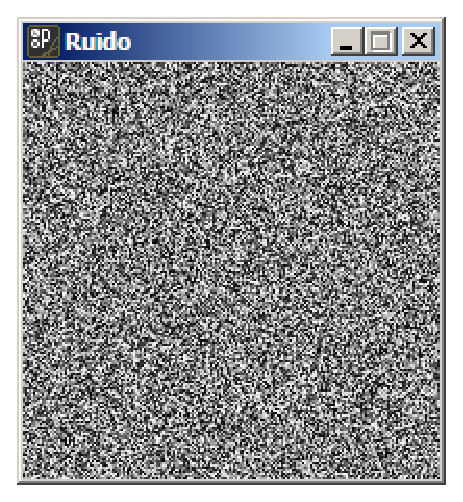
\includegraphics[width=4cm]{images/ruido.eps}
	\caption{Utilização de Matrizes: Ruído}
	\label{fig:ruido}
\end{figure}

\begin{lstlisting}
int ecra[][];

void setup() {
    size(200, 200);
    
    ecra = new int[200][200];
    
    // inicializar a matriz
    for (int i = 0; i < 200; i++) {
        for (int j = 0; j < 200; j++) {
            ecra[i][j] = (int)random(255);
        }
    }
}


void draw() { 
    // desenhar um ponto por cada elemento da matriz
    for (int i = 0; i < 200; i++) {
        for (int j = 0; j < 200; j++) {
            stroke(ecra[i][j]);
            point(j, i);
        }
    }    
}
\end{lstlisting}



\section{Exercícios}

\begin{enumerate}
\item \label{exe_5_ciclos}
* Escreva os programas para resolver os seguintes problemas:
\begin{enumerate}
\item Somar todos os elementos de um vector com 100 inteiros.

\item Somar todos os elementos, positivos, de um vector com 100 inteiros.

\item Somar todos os elementos, maiores do que 10 e inferiores a 20, de um vector com 100 inteiros.

\item Determinar a média dos valores de uma matriz de reais.

\item Dada uma matriz A, de números inteiros, criar uma segunda matriz, B, da seguinte forma: cada posição B[linha][coluna] 
é igual à média das 4 posições adjacentes à posição correspondente na matriz A.

\item Determinar se um número é primo.

\item Determinar o máximo de um conjunto de 20 números.

\item Determinar o mínimo de um conjunto de 20 números.

\end{enumerate}


\item 
Recrie \textbf{um} dos seguintes programas (ver site da cadeira) e publique-os:
\begin{itemize}
	\item ``Círculos''
	\item ``Linhas''
\end{itemize}

\item Recrie o programa ``Bolas Cadentes'' (ver site da cadeira) e publique-o.
\end{enumerate}